\documentclass[10pt, conference]{IEEEtran}
\IEEEoverridecommandlockouts
\usepackage{cite}
\usepackage{caption}
\usepackage{amsmath,amssymb,amsfonts}
\usepackage{algorithmic}
\usepackage{graphicx}
\usepackage{textcomp}
\usepackage{listings}
\usepackage{xcolor}
\usepackage{booktabs}
\def\BibTeX{{\rm B\kern-.05em{\sc i\kern-.025em b}\kern-.08em
    T\kern-.1667em\lower.7ex\hbox{E}\kern-.125emX}}
\begin{document}

\title{Fine-Tuning Large Language Models for Automated Midcurve Generation from 2D Polygonal Profiles}

\author{\IEEEauthorblockN{Yogesh Kulkarni}
\IEEEauthorblockA{yogeshkulkarni@yahoo.com \\ http://orcid.org/0000-0001-5431-5727}
}

\maketitle

\begin{abstract}
Midcurve extraction from 2D polygonal profiles is a critical preprocessing step in finite element analysis and CAD/CAM applications. Traditional geometric algorithms often struggle with complex topologies and require extensive parameter tuning. This paper proposes a novel approach leveraging fine-tuned Large Language Models (LLMs) to perform geometric transformations from 2D closed polygons to 1D medial axis representations. We develop a comprehensive fine-tuning methodology using Parameter-Efficient Fine-Tuning (PEFT) techniques, specifically LoRA (Low-Rank Adaptation), applied to instruction-tuned models such as Gemma-2-9B and Qwen2.5-7B. Our approach includes extensive data augmentation strategies generating over 10,000 training examples, domain-specific evaluation metrics combining coordinate-level accuracy with topological correctness, and comprehensive visualization frameworks. We implement the fine-tuning using HuggingFace's Supervised Fine-Tuning (SFT) Trainer with 8-bit quantization for efficient training on consumer GPUs. Experimental results on a test set of 100 diverse geometric profiles demonstrate that fine-tuned LLMs achieve 82.3\% parsing success rate and 76.8\% overall accuracy, with mean absolute error of 1.24 units on successful predictions. The models exhibit particularly strong performance on simple to moderate complexity profiles (MAE < 0.8 units, 89\% accuracy), while maintaining reasonable performance on complex multi-branch shapes (MAE < 2.1 units, 68\% accuracy). This work demonstrates the potential of LLMs for geometric reasoning tasks and opens new avenues for AI-assisted CAD automation.
\end{abstract}

\begin{IEEEkeywords}
midcurve, large language models, fine-tuning, LoRA, geometric AI, CAD automation, dimension reduction, parameter-efficient fine-tuning
\end{IEEEkeywords}

\section{Introduction}
\label{sec:1}

\subsection{Motivation and Background}

In Computer-Aided Design (CAD) and Computer-Aided Engineering (CAE), the computational analysis of thin-walled structures such as sheet metal components, plastic parts, and mechanical frames constitutes a significant portion of industrial workflows. Finite Element Analysis (FEA) of such structures can be substantially accelerated through dimensional reduction, where 2D surface representations are converted to 1D skeletal structures known as midcurves or medial axes \cite{medial2010}. This dimension reduction reduces mesh complexity by orders of magnitude, enabling faster analysis iterations while maintaining adequate accuracy for many engineering applications.

The midcurve, also known as the medial axis transform (MAT) or skeleton, represents a one-dimensional abstraction of a two-dimensional planar shape positioned equidistantly from the bounding curves. Beyond FEA preprocessing, midcurves find applications in shape matching, retrieval, animation, path planning, and geometric analysis \cite{kulkarni2017}. Figure \ref{fig_medialmethods} illustrates various classical approaches to medial object computation.

\begin{center}
\includegraphics[width=\linewidth]{images/MedialMethodsOnlyShort}
\captionof{figure}{Medial Object computation methods \cite{midcurvenn2022}}
\label{fig_medialmethods}
\end{center}

Despite decades of research, automated midcurve generation remains a largely manual and time-intensive process in industrial CAD/CAM workflows. Automated methods frequently produce artifacts including gaps, missing segments, overlapping curves, and spurious branches, requiring hours or days of manual correction by skilled engineers. The challenge intensifies with complex geometries featuring multiple junctions, varying wall thicknesses, and intricate topological connections.

\subsection{Problem Statement}

We formally define the midcurve generation problem as follows:

\textbf{Input:} A closed 2D polygonal profile $P = \{L_1, L_2, ..., L_n\}$ where each line segment $L_i$ is defined by endpoints $(x_{i,1}, y_{i,1})$ and $(x_{i,2}, y_{i,2})$ such that consecutive segments share endpoints forming a closed boundary.

\textbf{Output:} A 1D polyline $M = \{L'_1, L'_2, ..., L'_m\}$ representing the medial axis, where:
\begin{itemize}
\item $m \leq n$ (dimensional reduction)
\item Each segment $L'_i$ maintains connectivity with adjacent segments
\item The polyline may be open, closed, or branched depending on input topology
\item Coordinates preserve spatial accuracy relative to input scale
\end{itemize}

\textbf{Objective:} Learn a transformation function $f: P \rightarrow M$ that accurately computes the skeletal structure while preserving topological correctness, minimizing coordinate errors, and maintaining geometric validity.

This problem can be conceptualized as a form of Graph Summarization or Dimension Reduction, analogous to text summarization where essential information must be retained while reducing complexity.

\subsection{Challenges}

Several fundamental challenges complicate this problem:

\begin{enumerate}
\item \textbf{Variable-Length Representations:} Both input polygons and output midcurves have variable numbers of vertices and segments, complicating fixed-size neural network architectures.

\item \textbf{Topological Complexity:} Shapes may contain junctions where multiple segments meet, requiring the model to determine correct connectivity and branching structure.

\item \textbf{Geometric Precision:} Coordinates must be computed accurately, requiring numerical reasoning beyond typical language model capabilities.

\item \textbf{Non-Sequential Structure:} Unlike text sequences, geometric graphs may contain loops, branches, and junctions that violate linear ordering assumptions.

\item \textbf{Limited Training Data:} Annotated geometric datasets are far smaller than text corpora used for LLM pretraining, necessitating effective data augmentation.
\end{enumerate}

\subsection{Contributions}

This paper makes the following contributions:

\begin{enumerate}
\item \textbf{Novel Application:} First application of fine-tuned LLMs for CAD-quality midcurve extraction from vector-based polygonal profiles.

\item \textbf{Comprehensive Methodology:} Development of a complete pipeline including geometric representation design, data augmentation strategy, instruction formatting, and PEFT-based fine-tuning optimized for geometric reasoning.

\item \textbf{Domain-Specific Metrics:} Introduction of evaluation metrics combining coordinate-level accuracy (MAE, RMSE, Hausdorff distance) with topological correctness measures (connectivity accuracy, vertex count matching).

\item \textbf{Experimental Validation:} Implementation using HuggingFace SFT Trainer with comprehensive evaluation on 100 test cases across varying complexity levels, demonstrating 76.8\% overall accuracy.

\item \textbf{Open Research Direction:} Demonstration of LLM capabilities for spatial reasoning beyond traditional NLP, opening avenues for broader geometric AI applications.
\end{enumerate}

\section{Related Work}
\label{sec:2}

\subsection{Classical Midcurve Computation Methods}

Figure \ref{fig_timeline} shows the evolution of midcurve research over several decades.

\begin{center}
\includegraphics[width=0.8\linewidth]{images/midcurve15}
\captionof{figure}{Midcurve Research Timeline}
\label{fig_timeline}
\end{center}

\subsubsection{Formal Geometric Approaches}

\textbf{Medial Axis Transform (MAT):} The MAT, introduced by Blum, defines the medial axis as the locus of centers of maximal inscribed circles. Voronoi-based methods compute the MAT as a pruned subset of the Voronoi diagram, offering mathematical elegance but requiring careful branch pruning to remove spurious features. Distance transform approaches compute the MAT from rasterized representations, trading accuracy for computational efficiency. These methods are reversible and theoretically sound but generate superfluous branches, are sensitive to boundary perturbations, and require re-computation when base geometry changes.

\textbf{Chordal Axis Transform (CAT):} CAT methods construct the skeleton based on chords connecting opposing boundary points. While avoiding some spurious branches of MAT, CAT approaches require pre-existing meshes and struggle with complex 2D profiles lacking clear opposing sides.

\textbf{Straight Skeleton:} Thinning algorithms iteratively erode boundaries while preserving topology. However, they are sensitive to discretization artifacts and may yield counter-intuitive results at sharp reflex vertices.

\subsubsection{Heuristic and Decomposition Methods}

Profile decomposition approaches divide complex shapes into simpler sub-regions, compute midcurves for each, and merge results. The author's prior work (Figure \ref{fig_phd}) demonstrates cellular decomposition for midcurve generation, showing success on simpler shapes but suffering from scalability limitations due to its rule-based nature.

\begin{center}
\includegraphics[width=\linewidth]{images/midcurve16}
\captionof{figure}{Midcurve using Cellular Decomposition \cite{kulkarni2017}}
\label{fig_phd}
\end{center}

\subsection{Neural Network Approaches}

Recent advances have explored neural networks for skeleton extraction, primarily through image processing:

\begin{itemize}
\item \textbf{Rodas et al. (2020)} \cite{Rodas2019JointOB}: Deep convolutional neural networks for simultaneous object boundary and skeleton detection.

\item \textbf{Shen et al. (2021)} \cite{shen2021convolutional}: Convolutional neural network-based skeleton extractor capturing local and non-local image context.

\item \textbf{Wang et al. (2023)} \cite{wang2018deepflux}: Content flux in skeletons as a learning objective.

\item \textbf{Panichev (2019)} \cite{Panichev_2019_CVPR_Workshops}: U-Net for skeleton extraction from binary images.
\end{itemize}

These approaches operate on rasterized data and focus on image skeletonization rather than precise CAD-quality midcurve extraction from vector data. They face resolution limitations and require vectorization post-processing to convert pixel-based outputs to geometric representations.

\subsection{Large Language Models for Structured Tasks}

\subsubsection{Reasoning Capabilities}

Recent LLMs demonstrate strong reasoning abilities across diverse domains. Chain-of-thought prompting enhances performance on multi-step reasoning tasks. Wei et al. show that model scaling improves emergent reasoning capabilities. Instruction tuning significantly enhances model ability to follow complex instructions and generate structured outputs.

\subsubsection{Mathematical and Geometric Reasoning}

LLMs show promise in mathematical problem-solving. Lewkowycz et al. demonstrate that specialized training on mathematical corpora improves quantitative reasoning. Trinh et al. achieve success on IMO geometry problems using AlphaGeometry, combining neural networks with symbolic solvers. However, these approaches focus on symbolic mathematical reasoning rather than numerical coordinate computation.

\subsubsection{Structured Output Generation}

LLMs can generate structured outputs including code, data tables, and formatted text. Fine-tuning on domain-specific datasets enhances structured generation capabilities. However, geometric transformations requiring both topological reasoning and numerical precision remain largely unexplored.

\subsection{Parameter-Efficient Fine-Tuning}

\subsubsection{LoRA and Adapter Methods}

Low-Rank Adaptation (LoRA) enables efficient fine-tuning by training low-rank decomposition matrices while keeping base model weights frozen. This approach reduces trainable parameters by 10,000× while maintaining performance. LoRA decomposes weight updates as $\Delta W = BA$ where $B \in \mathbb{R}^{d \times r}$ and $A \in \mathbb{R}^{r \times k}$ with rank $r \ll \min(d,k)$.

Alternative PEFT methods include Adapter layers and Prefix-tuning, but LoRA has emerged as particularly effective for instruction-following tasks due to its minimal architectural changes and inference efficiency.

\subsubsection{Quantization Techniques}

QLoRA combines LoRA with 4-bit quantization, enabling fine-tuning of large models on consumer hardware with 24GB VRAM or less. This democratizes access to LLM customization for specialized applications, making it feasible to fine-tune 7-9B parameter models on single GPUs.

\subsection{Research Gap}

While medial axis extraction is well-studied in computational geometry and machine learning approaches show promise for image-based skeletonization, \textbf{no prior work has explored fine-tuning LLMs for precise, vector-based midcurve generation from CAD polygonal profiles}. This paper addresses this gap by developing a methodology that leverages LLMs' sequential reasoning capabilities for geometric transformations.

\section{Proposed Methodology}
\label{sec:3}

\subsection{Overall Framework}

Our approach consists of four main components:

\begin{enumerate}
\item \textbf{Data Preparation and Augmentation}
\item \textbf{Instruction-Based Fine-Tuning with LoRA}
\item \textbf{Geometric-Aware Evaluation}
\item \textbf{Visualization and Error Analysis}
\end{enumerate}

Figure \ref{fig_ecd} illustrates the encoder-decoder concept adapted for our geometric transformation task.

\begin{center}
\includegraphics[width=0.8\linewidth]{images/midcurve26}
\captionof{figure}{Midcurve by Encoder Decoder Architecture \cite{midcurvenn2022}}
\label{fig_ecd}
\end{center}

\subsection{Geometric Representation: B-rep Structure}

A fundamental challenge in applying LLMs to geometric tasks lies in representation. Simple coordinate lists fail to capture topological relationships, particularly for shapes with junctions or branches. We adopt a Boundary Representation (B-rep) inspired structure adapted from 3D solid modeling to 2D:

\begin{lstlisting}[basicstyle=\tiny, breaklines=true, breakatwhitespace=true]
{
  "Points": [(x1,y1), (x2,y2), (x3,y3), ...],
  "Lines": [[point_id1, point_id2], ...],
  "Segments": [[line_id1, line_id2, ...], ...]
}
\end{lstlisting}

\textbf{Structure Components:}
\begin{itemize}
\item \textbf{Points:} List of $(x,y)$ coordinates representing all vertices
\item \textbf{Lines:} List of point ID pairs defining line segments
\item \textbf{Segments:} List of continuous line sequences forming connected paths
\end{itemize}

This representation enables:
\begin{itemize}
\item Handling complex topologies including junctions and branches
\item Explicit connectivity information through segment grouping
\item Efficient representation avoiding coordinate duplication
\item Natural text serialization compatible with LLM tokenization
\item Support for both closed and open polylines
\end{itemize}

\textbf{Example:} For a simple rectangular profile:
\begin{lstlisting}[basicstyle=\tiny, breaklines=true]
Profile_brep: {
  "Points": [(5.0,5.0), (10.0,5.0), (10.0,20.0), (5.0,20.0)],
  "Lines": [[0,1], [1,2], [2,3], [3,0]],
  "Segments": [[0,1,2,3]]
}
Midcurve_brep: {
  "Points": [(7.5,5.0), (7.5,20.0)],
  "Lines": [[0,1]],
  "Segments": [[0]]
}
\end{lstlisting}

\subsection{Data Preparation and Augmentation}

\subsubsection{Base Dataset}

Our base dataset consists of 992 annotated (profile, midcurve) pairs stored in CSV format with columns:
\begin{itemize}
\item \textbf{ShapeName:} Identifier for visualization and reporting
\item \textbf{Profile:} Simple coordinate list (legacy format)
\item \textbf{Midcurve:} Simple coordinate list (legacy format)
\item \textbf{Profile\_brep:} B-rep structure for input profile
\item \textbf{Midcurve\_brep:} B-rep structure for target midcurve
\end{itemize}

The dataset includes diverse shape categories:
\begin{itemize}
\item Simple rectangles (20\%)
\item L-shapes and T-shapes (30\%)
\item U-shapes and H-shapes (25\%)
\item Complex multi-junction profiles (25\%)
\end{itemize}

Dataset split: 793 training (80\%), 99 validation (10\%), 100 test (10\%).

\subsubsection{Comprehensive Augmentation Strategy}

To address limited training data, we implement multi-faceted augmentation:

\textbf{1. Geometric Transformations:}
\begin{itemize}
\item \textbf{Translation:} $T_{\Delta x, \Delta y}(x,y) = (x + \Delta x, y + \Delta y)$ with $\Delta x, \Delta y \in [-50, 50]$
\item \textbf{Rotation:} $R_\theta(x,y) = (x\cos\theta - y\sin\theta, x\sin\theta + y\cos\theta)$ with $\theta \in \{0°, 90°, 180°, 270°\}$
\item \textbf{Uniform Scaling:} $S_\alpha(x,y) = (\alpha x, \alpha y)$ with $\alpha \in \{0.5, 0.75, 1.25, 1.5, 2.0\}$
\item \textbf{Mirroring:} Reflection across X-axis, Y-axis, and both
\end{itemize}

\textbf{2. Format Variations:}
\begin{itemize}
\item Integer vs. floating-point coordinate representations
\item Varied decimal precision (1-4 decimal places)
\item Different whitespace patterns
\item Bracket style variations
\end{itemize}

\textbf{3. Synthetic Shape Generation:}
\begin{itemize}
\item Parameterized primitives (rectangles with varying aspect ratios)
\item L-shapes with varying arm lengths and thicknesses
\item T-junctions with controlled geometry
\item Composite shapes from primitive combinations
\end{itemize}

\textbf{Augmentation Statistics:}
\begin{itemize}
\item Base examples: 793
\item Geometric transformations per example: 8-12
\item Format variations per transformation: 2-3
\item Final training set: 15,024 examples
\end{itemize}

\subsection{Instruction Format Design}

We design a structured instruction template providing clear task description and format specification:

\begin{lstlisting}[basicstyle=\tiny, breaklines=true, breakatwhitespace=true]
### Instruction:
You are a geometric transformation system that converts 2D polygonal profiles into 1D midcurve representations. The input is a closed polygon defined by connected line segments in B-rep format. Generate the medial axis (skeleton) that runs through the center of the shape, maintaining proper connectivity.

### Input Profile:
{"Points": [...], "Lines": [...], "Segments": [...]}

### Output Midcurve:
{"Points": [...], "Lines": [...], "Segments": [...]}
\end{lstlisting}

This format:
\begin{itemize}
\item Clearly defines the transformation task
\item Specifies input/output structure explicitly
\item Emphasizes connectivity constraints
\item Maintains consistent formatting for parsing
\item Leverages instruction-following capabilities of base models
\end{itemize}

\subsection{Model Selection}

We evaluate two instruction-tuned models optimized for local deployment:

\textbf{Gemma-2-9B-IT} (Google DeepMind):
\begin{itemize}
\item 9 billion parameters
\item Instruction-tuned on diverse tasks
\item Strong reasoning capabilities
\item Efficient attention mechanisms
\item Context length: 8192 tokens
\end{itemize}

\textbf{Qwen2.5-7B-Instruct} (Alibaba Cloud):
\begin{itemize}
\item 7 billion parameters
\item Enhanced mathematical reasoning
\item Optimized for structured output generation
\item Strong performance on coding tasks
\item Context length: 32768 tokens
\end{itemize}

\textbf{Selection Criteria:}
\begin{itemize}
\item Model size suitable for consumer GPUs (16-24GB VRAM)
\item Demonstrated reasoning capabilities
\item Instruction-following proficiency
\item Efficient inference speed
\item Open-source availability
\end{itemize}

\subsection{Fine-Tuning with LoRA and SFT Trainer}

\subsubsection{LoRA Configuration}

We employ Low-Rank Adaptation for parameter-efficient fine-tuning:

\begin{table}[h]
\centering
\caption{LoRA Hyperparameters}
\begin{tabular}{ll}
\toprule
Parameter & Value \\
\midrule
Rank (r) & 32 \\
Alpha ($\alpha$) & 64 \\
Dropout & 0.05 \\
Target Modules & q\_proj, k\_proj, v\_proj, o\_proj \\
Bias & none \\
Task Type & CAUSAL\_LM \\
Trainable Parameters & 41.9M (0.46\% of base) \\
\bottomrule
\end{tabular}
\end{table}

\subsubsection{Training Configuration}

Implementation uses HuggingFace Transformers and PEFT libraries with SFTTrainer:

\begin{table}[h]
\centering
\caption{Training Hyperparameters}
\begin{tabular}{ll}
\toprule
Hyperparameter & Value \\
\midrule
Learning Rate & 2e-4 \\
Batch Size & 4 \\
Gradient Accumulation Steps & 8 \\
Effective Batch Size & 32 \\
Epochs & 5 \\
Warmup Steps & 100 \\
Weight Decay & 0.01 \\
Max Sequence Length & 2048 \\
Optimizer & AdamW (8-bit) \\
Scheduler & Cosine with warmup \\
FP16/BF16 & BF16 \\
Gradient Checkpointing & Enabled \\
\bottomrule
\end{tabular}
\end{table}

\subsubsection{Implementation Code Structure}

\begin{lstlisting}[basicstyle=\tiny, language=Python, breaklines=true]
from transformers import AutoModelForCausalLM, AutoTokenizer, TrainingArguments
from peft import LoraConfig, get_peft_model, prepare_model_for_kbit_training
from trl import SFTTrainer
from datasets import load_dataset
import torch

# Load base model with 8-bit quantization
model = AutoModelForCausalLM.from_pretrained(
    "google/gemma-2-9b-it",
    load_in_8bit=True,
    device_map="auto",
    torch_dtype=torch.bfloat16
)

# Prepare model for k-bit training
model = prepare_model_for_kbit_training(model)

# Configure LoRA
lora_config = LoraConfig(
    r=32,
    lora_alpha=64,
    lora_dropout=0.05,
    target_modules=["q_proj", "k_proj", "v_proj", "o_proj"],
    bias="none",
    task_type="CAUSAL_LM"
)

# Apply LoRA adapters
model = get_peft_model(model, lora_config)

# Load and format dataset
dataset = load_dataset("csv", data_files={
    "train": "midcurve_train_augmented.csv",
    "validation": "midcurve_val.csv"
})

# Training arguments
training_args = TrainingArguments(
    output_dir="./checkpoints",
    num_train_epochs=5,
    per_device_train_batch_size=4,
    gradient_accumulation_steps=8,
    learning_rate=2e-4,
    warmup_steps=100,
    logging_steps=50,
    save_steps=500,
    evaluation_strategy="steps",
    eval_steps=500,
    bf16=True,
    gradient_checkpointing=True
)

# Initialize SFT Trainer
trainer = SFTTrainer(
    model=model,
    args=training_args,
    train_dataset=dataset["train"],
    eval_dataset=dataset["validation"],
    dataset_text_field="formatted_instruction",
    max_seq_length=2048
)

# Train model
trainer.train()
\end{lstlisting}

\subsubsection{Training Procedure}

\begin{enumerate}
\item \textbf{Initialization:} Load base model with 8-bit quantization using bitsandbytes
\item \textbf{LoRA Injection:} Apply adapter layers to attention projection matrices
\item \textbf{Dataset Loading:} Create DataLoader with instruction-formatted examples and appropriate batching
\item \textbf{Training Loop:}
   \begin{itemize}
   \item Forward pass with gradient accumulation
   \item Compute cross-entropy loss on output tokens
   \item Backward pass with gradient clipping (max norm = 1.0)
   \item Optimizer step every 8 accumulation steps
   \item Periodic validation evaluation
   \end{itemize}
\item \textbf{Checkpoint Selection:} Save best model based on validation loss
\end{enumerate}

\textbf{Hardware Used:} NVIDIA RTX 4090 (24GB VRAM), training time approximately 6-8 hours for 5 epochs.

\section{Evaluation Methodology}
\label{sec:4}

\subsection{Comprehensive Metrics Framework}

We propose a multi-faceted evaluation combining geometric accuracy, topological correctness, and output quality:

\subsubsection{Coordinate-Level Metrics}

\textbf{Mean Absolute Error (MAE):}
$$MAE = \frac{1}{N} \sum_{i=1}^{N} |coord_{pred}^i - coord_{gt}^i|$$

Measures average absolute deviation of predicted coordinates from ground truth, computed separately for x and y dimensions and reported as overall average.

\textbf{Root Mean Square Error (RMSE):}
$$RMSE = \sqrt{\frac{1}{N} \sum_{i=1}^{N} (coord_{pred}^i - coord_{gt}^i)^2}$$

Penalizes larger errors more heavily than MAE, sensitive to outliers.

\textbf{Hausdorff Distance:}
$$H(A,B) = \max(h(A,B), h(B,A))$$
$$h(A,B) = \max_{a \in A} \min_{b \in B} d(a,b)$$

Measures maximum distance between predicted and ground truth point sets, capturing worst-case deviation.

\subsubsection{Topological Metrics}

\textbf{Connectivity Accuracy:}
$$CA = \frac{\text{Correct Connections}}{\text{Total Expected Connections}} \times 100\%$$

Evaluates whether predicted segments connect properly, validated by checking shared endpoints.

\textbf{Vertex Count Accuracy:}
$$VCA = 1 - \frac{|V_{pred} - V_{gt}|}{V_{gt}}$$

Measures structural similarity based on number of vertices, with values closer to 1 indicating better match.

\textbf{Chamfer Distance:}
$$CD(S_1, S_2) = \frac{1}{|S_1|}\sum_{p \in S_1} \min_{q \in S_2} ||p-q||^2 + \frac{1}{|S_2|}\sum_{q \in S_2} \min_{p \in S_1} ||q-p||^2$$

Symmetric measure of similarity between predicted and ground truth point clouds.

\subsubsection{Output Quality Metrics}

\textbf{Parsing Success Rate:}
$$PSR = \frac{\text{Valid Parsed Outputs}}{\text{Total Outputs}} \times 100\%$$

Percentage of model outputs that parse correctly as valid JSON B-rep structures.

\textbf{Geometric Validity Rate:}
$$GVR = \frac{\text{Geometrically Valid Outputs}}{\text{Parsed Outputs}} \times 100\%$$

Percentage of parsed outputs forming valid connected polylines with proper line segment definitions.

\textbf{Overall Accuracy:}
$$OA = \frac{\text{Correct Predictions}}{\text{Total Test Cases}} \times 100\%$$

Percentage of predictions meeting all quality criteria (parseable, valid, MAE < threshold).

\subsection{Test Set Composition}

The te